 \begin{center}
    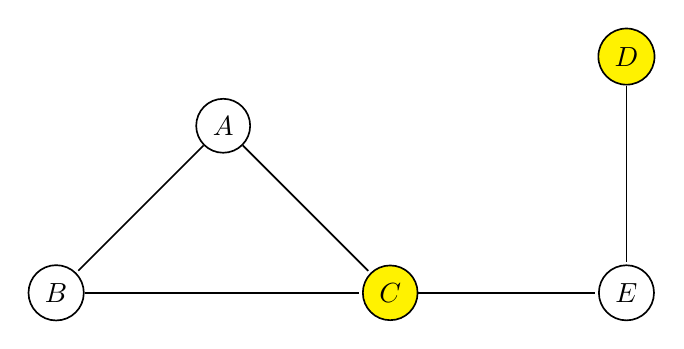
\begin{tikzpicture}[
            thick, 
            main/.style = {draw, circle}, 
            > = stealth, % arrow head style
            shorten > = 1pt, % don't touch arrow head to node
            auto,
            node distance = 3cm, % distance between nodes
            semithick % line style
        ]
        \node[main] (a) {$A$};
        \node[main] (b) [below left of=a] {$B$};
        \node[main] (c) [below right of=a, fill=yellow] {$C$}; 
        \node[main] (e) [right of=c] {$E$};
        \node[main] (d) [above of=e, fill=yellow] {$D$};

        \path[-] (a) edge node {} (b);
        \path[-] (a) edge node {} (c);
        \path[-] (b) edge node {} (c);
        \path[-] (c) edge node {} (e);
        \path[-] (d) edge node {} (e);
    \end{tikzpicture} 
\end{center}